\documentclass{article}
\usepackage{tikz}
\usetikzlibrary{arrows.meta}

\begin{document}

\section*{A TikZ figure}

\begin{center}
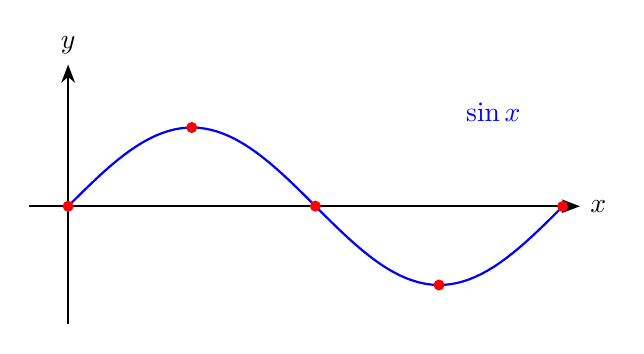
\begin{tikzpicture}[>=Stealth, thick]
  % axes
  \draw[->] (-0.5,0) -- (6.5,0) node[right] {$x$};
  \draw[->] (0,-1.5) -- (0,1.8) node[above] {$y$};
  % a sine wave
  \draw[blue, domain=0:6.28, samples=80] plot (\x, {sin(\x r)});
  \node[blue] at (5.4,1.2) {$\sin x$};
  % a few points on it
  \foreach \t in {0, 1.57, 3.14, 4.71, 6.28}
    \fill[red] (\t, {sin(\t r)}) circle (2pt);
\end{tikzpicture}
\end{center}

Change the colour, the domain or the number of samples, and the figure
is drawn again as you type.

\end{document}
